\documentclass[conference]{IEEEtran}
\IEEEoverridecommandlockouts
% The preceding line is only needed to identify funding in the first footnote. If that is unneeded, please comment it out.
\usepackage{cite}
\usepackage{amsmath,amssymb,amsfonts}
\usepackage{algorithmic}
\usepackage{graphicx}
\usepackage{textcomp}
\usepackage{xcolor}
\usepackage{hyperref}
\usepackage[brazil]{babel}
% Definindo novas cores
\definecolor{verde}{rgb}{0,0.5,0}
% Configurando layout para mostrar codigos C++

\def\BibTeX{{\rm B\kern-.05em{\sc i\kern-.025em b}\kern-.08em
    T\kern-.1667em\lower.7ex\hbox{E}\kern-.125emX}}
    
\begin{document}

\title{Programação Orientada a Objetos: Operações Bancárias em C++\\
{\footnotesize Projeto Final - Programação III}
\thanks{}
}


\author{\IEEEauthorblockN{Rubens Heryson de Lima Lavor}
\IEEEauthorblockA{\textit{Centro Tecnológico de Joinville} \\
\textit{Universidade Federal de Santa Catarina-UFSC}\\
Joinville, Brasil \\
rubens.lavor@grad.ufsc.br}
\and
{Thaiz Antunes Izidoro}\\
\IEEEauthorblockA{\textit{Centro Tecnológico de Joinville} \\
\textit{Universidade Federal de Santa Catarina-UFSC}\\
Joinville, Brasil \\
thaiz.izidoro@grad.ufsc.br}
}


\maketitle

\begin{abstract}
    Este projeto visa demonstrar os principais conceitos de orientação a objeto usando a linguagem C++; são eles: Classe, Encapsulamento, Agregação e Composição, Templates, Sobrecarga de operador, Herança e Polimorfismo. Por meio  de operações bancárias tais como abertura de contas, transferências, demonstrativos bancários (extratos), entre outros. 
\end{abstract}

\begin{IEEEkeywords}
    C++, Programação, Orientação a Objetos, Operações Bancárias.
\end{IEEEkeywords}

\section{Introdução}
Este relatório tem o objetivo de detalhar a lógica de funcionamento do programa, apresentar as principais classes e demonstrar os coceitos usados  para o desenvolvido das operações do sistema bancário, feito para o trabalho final da disciplina de programação 3. Todo o código está documentado nos arquivos de cabeçalho.

\section{Desenvolvimento}

\subsection{Classe Conta}
\begin{figure}[htbp]
    \centering
    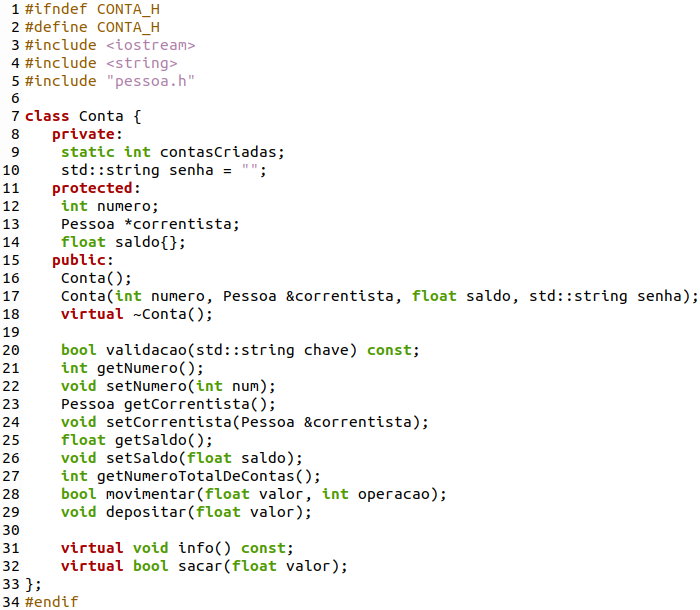
\includegraphics[width=8.8cm]{../img/Conta.png}
    \caption{Arquivo de cabeçalho conta.h}
    \label{fig_conta}
\end{figure}
A classe Conta define um tipo de dado abstrato para a criação da estrutura de classes de contas bancárias, é a estrutura central do projeto e classe base para as classes derivadas ContaComum, ContaEspecial e ContaPoupanca, ou seja, estas três, herdam as funcionalidades de Conta. Nela encontramos atributos e métodos comuns a todas as contas (e o que esperamos que elas tenham no mundo real). Exemplos de atributos presentes: senha, número da conta, saldo; exemplos de métodos: depositar, sacar, entre outras.

Conceitos fundamentais de OO a partir da Classe Conta:
\begin{enumerate}
    \item \textbf{Encapsulamento}: Em linguagens orientadas a objeto, é a capacidade de ocultação de detalhes de implementação por parte de entidades de manipulação de dados, por meio dos especificadores de acesso, em C++ são três: \textbf{public}, \textbf{private} e \textbf{protected}. Cada atributo oferece um nível de ocultação para membros de classes.
    \item \textbf{Agregação}: Conta possui uma referência para a classe Pessoa, trata-se de uma associação na forma de agregação, pois o objeto do tipo Pessoa não deixa de existir quando quando o objeto do tipo Conta, associado a ele, é destruído. Com isso um objeto Conta, por meio dos métodos presentes na classe Pessoa, pode ter acesso ao nome e CPF do correntista.
    \begin{figure}[htbp]
        \centering
        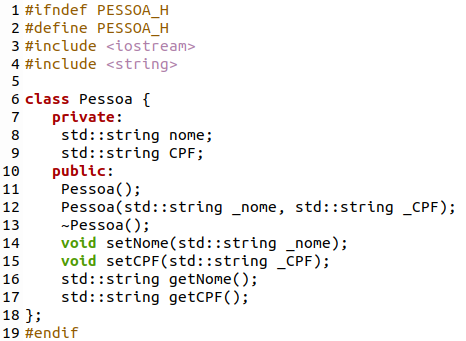
\includegraphics[width=7.5cm]{../img/Pessoa.png}
        \caption{Arquivo de cabeçalho pessoa.h}
        \label{fig_pessoa}
    \end{figure}
    \item \textbf{Herança}: Herança é um dos pontos chave de programação orientada a objetos. Ela fornece meios de promover a extensibilidade do código, a reutilização e uma maior coerência lógica no modelo de implementação.
    \begin{figure}[htbp]
        \centering
        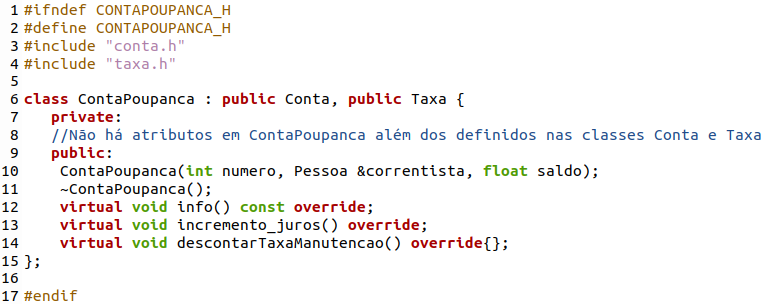
\includegraphics[width=8.8cm]{../img/ContaPoupanca.png}
        \caption{Arquivo de cabeçalho contaPoupanca.h}
        \label{fig_contaPoupanca}
    \end{figure}
    
    \item \textbf{Polimorfismo}: O polimorfismo em C++ se apresenta sob diversas formas diferentes, desde as mais simples, como funções com mesmo nome e lista de parâmetros diferentes, até as mais complexas como funções virtuais, cujas formas de execução são dependentes da classe a qual o objeto pertence e são identificadas em tempo de execução.
    No método sacar, por exemplo, o polimorfismo é necessário, pois a classe ContaEspecial permite que o correntista saque um valor além do saldo, trata-se de um limite especial que esse tipo de conta oferece. Mesmo com o saldo zerado, é possível realizar um saque até determinado valor. Isso já não acontece, por exemplo, em ContaPoupanca, onde não é possível sacar valores além do saldo em conta, cada classe apresenta um comportamento distinto para a funcionalidade sacar.
    \end{enumerate}

    \subsection{Classe Movimento}
    A classe Movimento registra todas as atividades de uma determinada conta. Sempre que uma nova transação é realizada, um objeto Movimento é criado e associado a conta correspondente. 
    \begin{figure}[htbp]
        \centering
        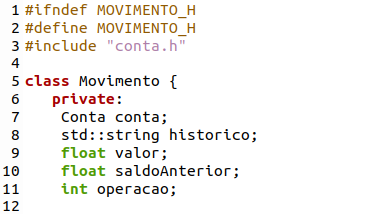
\includegraphics[width=7cm]{../img/Movimento.png}
        \caption{Arquivo de cabeçalho movimento.h}
        \label{fig_movimento}
    \end{figure}

    A relação entre as classes Movimento e Conta é na forma de uma agregação. Os atributos “historico”,”valor” e “operacao” armazenam, a descrição da transação, valor da transação, se é saque ou depósito; respectivamente.

    \subsection{Classe Transacao}
    Transacao controla operações de movimentações bancárias. Mesmo sendo totalmente possível um objeto ContaComum, por exemplo, realizar um saque ou depósito, no código do projeto isso é feito apenas por meio de um objeto do tipo Transacao. Pois assim é possível criar um objeto Movimento e registrar as atividades bancárias realizadas.
    \begin{figure}[htbp]
        \centering
        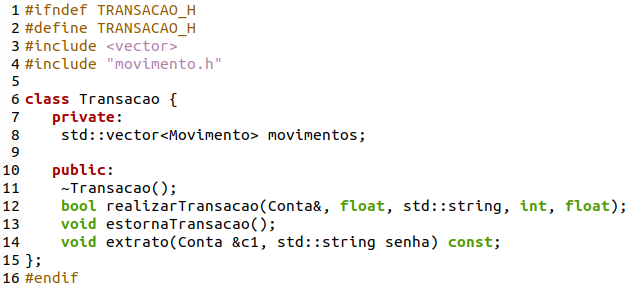
\includegraphics[width=8.8cm]{../img/Transacao.png}
        \caption{Arquivo de cabeçalho Transacao.h}
        \label{fig_Transacao}
    \end{figure}

    A classe Transacao é composta por objetos do tipo Movimento, existe uma relação entre a classe Transacao e a classe Movimento na forma de uma composição, ou seja, no momento em que uma instância de Transacao deixar de existir, serão destruídas todas as instâncias de Movimento, associadas ao objeto. 
O método “realizarTransacao” cria e adiciona um objeto do tipo Movimento ao vector movimentos, caso a operação seja realizada.

\subsection{Classe Lista}

Template de classe e sobrecarga de operador

\begin{figure}[htbp]
    \centering
    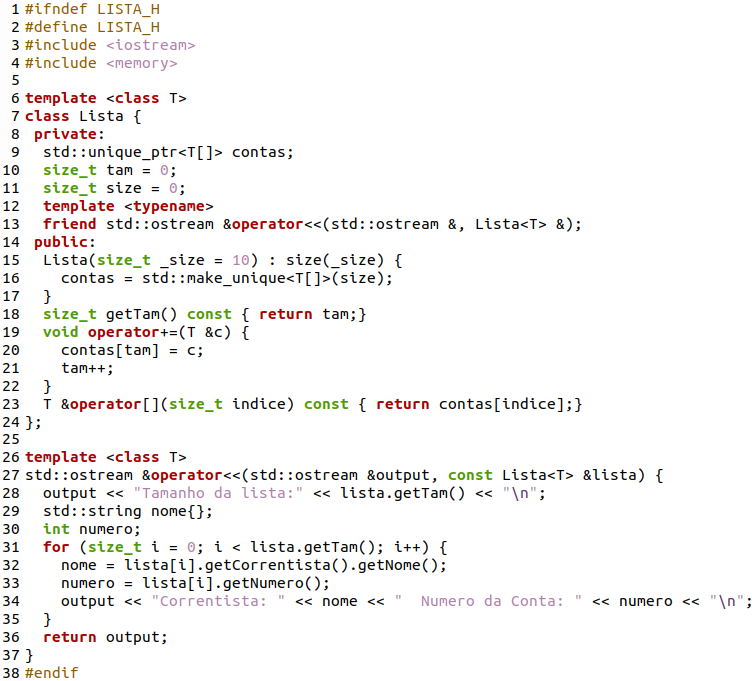
\includegraphics[width=8.8cm]{../img/Lista.png}
    \caption{Arquivo de cabeçalho Lista.h}
    \label{fig_Lista}
\end{figure}

A classe Lista é composta por elementos do tipo T a ser definido pelo compilador em tempo de execução. Apesar do C++ ser uma linguagem fortemente tipada, ela permite que isso seja feito através dos templates. Além disso outro conceito muito importante presente nesta classe é o de sobrecarga de operador. Os operadores sobrecarregados são += , [] e $ << $. Por meio das sobrecargas a classe provém métodos de adicionar um elemento ao array e imprime no terminal informações referentes a esses elementos.


\section{Discussão}
O arquivo main.cpp do projeto, exemplifica o uso das classe apresentadas anteriormeente, da segunite forma:
\begin{itemize}
    \item Cria-se 3 objetos do tipo pessoa, passando nome e numero do CPF.
    \item Em seguida 3 contas, comum, especial e poupança, passando um objeto pessoa, saldo inicial e o número da conta. Conta também espera uma senha, que se não for passada, por padrão é "123".
    \item Após a criação das contas, é criada uma lista do tipo Conta e tamanho 5, nela são colocadas as 3 contas. Nesse ponto fica clara a função do operador sobrecarregado += . O operador de saida $<<$ também é usado em sobrecarga.
    \item Por fim um objeto do tipo Transacao é instaciado e 3 movimentações são feitas: José paga o telefone, Maria recebe o salário e Lúcia faz um empréstimo. Depois é emitido um extrato de cada correntista.
    \end{itemize}
    \begin{figure}[htbp]
        \centering
        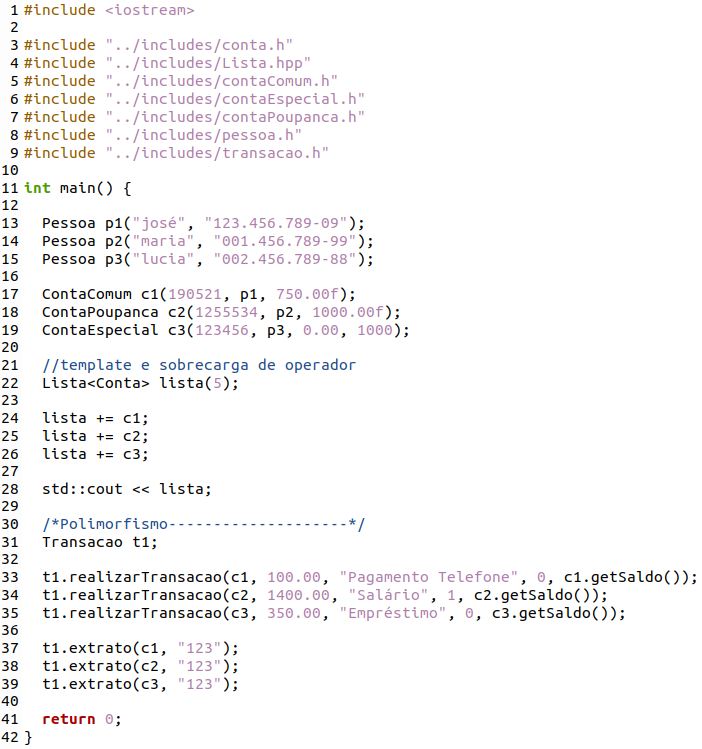
\includegraphics[width=8.8cm]{../img/main.png}
        \caption{main.cpp}
        \label{fig_main}
    \end{figure}

    O programa não recebe nenhuma entrada, apenas imprime demonstrativos das suas funcionalidades. Ele é simples no seu entendimento e implementação, porém contempla todos os conceitos propostos de orientação a objeto.

    Saída do programa após rodar o arquivo executável:
    \begin{figure}[htbp]
        \centering
        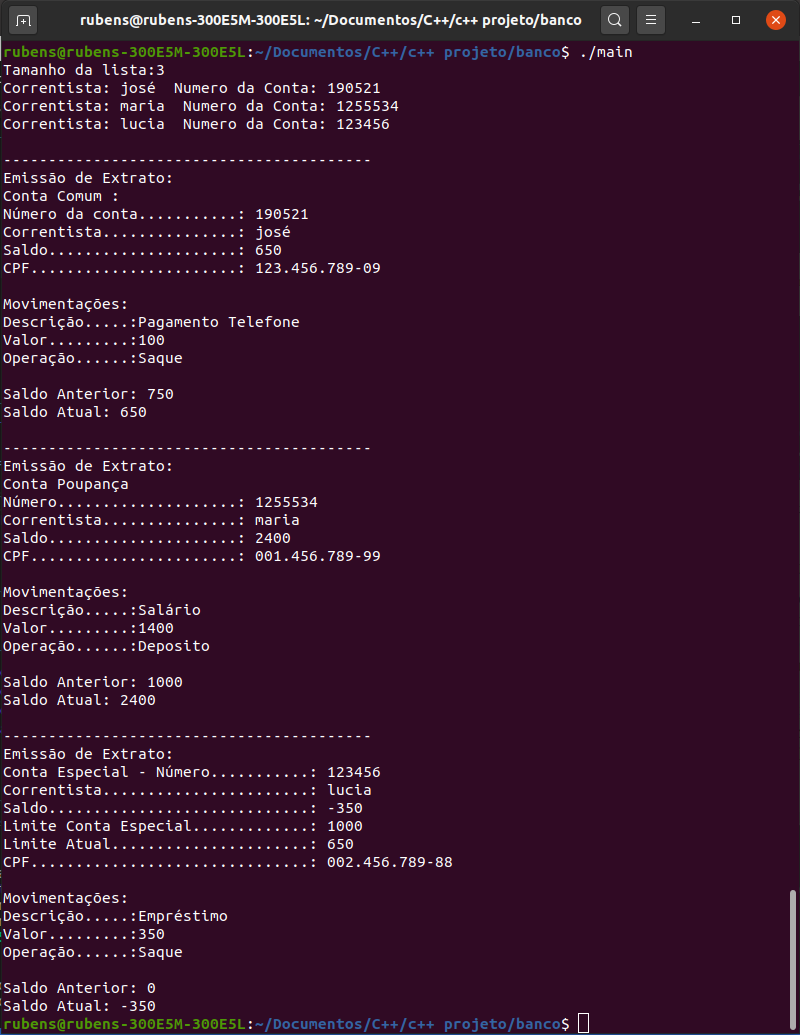
\includegraphics[width=8.8cm]{../img/exec.png}
        \caption{Saída do Programa}
        \label{fig_programa}
    \end{figure}

    \subsection{Ambiente de Desenvolmento}

    O código foi desenvolvido e testado na IDE VScode em máquina com o sistema operacinal 
    Ubuntu 20.04 LTS, compilador GCC (GNU Compiler Collection) na versão 9.3.0.

    \subsection{Uso de Memória, Flags para Compilação e Makefile}
        O uso de memória foi verificado usando valgrind. Valgrind é um software livre que auxilia o trabalho de depuração de programas. Ele possui ferramentas que detectam erros decorrentes do uso incorreto da memória dinâmica, como por exemplo os vazamentos de memória, alocação e desalocação incorretas e acessos a áreas inválidas
        
        De maniera bem simplista um makefile é um arquivo de texto que contém instruções sobre como compilar e executar (ou construir) um conjunto de arquivos de código-fonte C ++.

        Flags usadas na compilação do projeto: -std=c++17 -Wall -Wextra -Werror 
    -Wshadow-Wconversion -Wcast-align -Wcast-qual -Wctor-dtor-privacy -Wdisabled-optimization -Wformat=2 -Winit-self -Wlogical-op -Wmissing-declarations -Wmissing-include-dirs -Wnoexcept -Wold-style-cast -Woverloaded-virtual -Wredundant-decls -Wsign-conversion -Wsign-promo -Wstrict-null-sentinel -Wstrict-overflow=5 -Wswitch-default -Wundef -Wno-unused

    \subsection{Demonstração de Funcionamento}

    Uso das flags mencionadas na compilação:
    \begin{figure}[htbp]
        \centering
        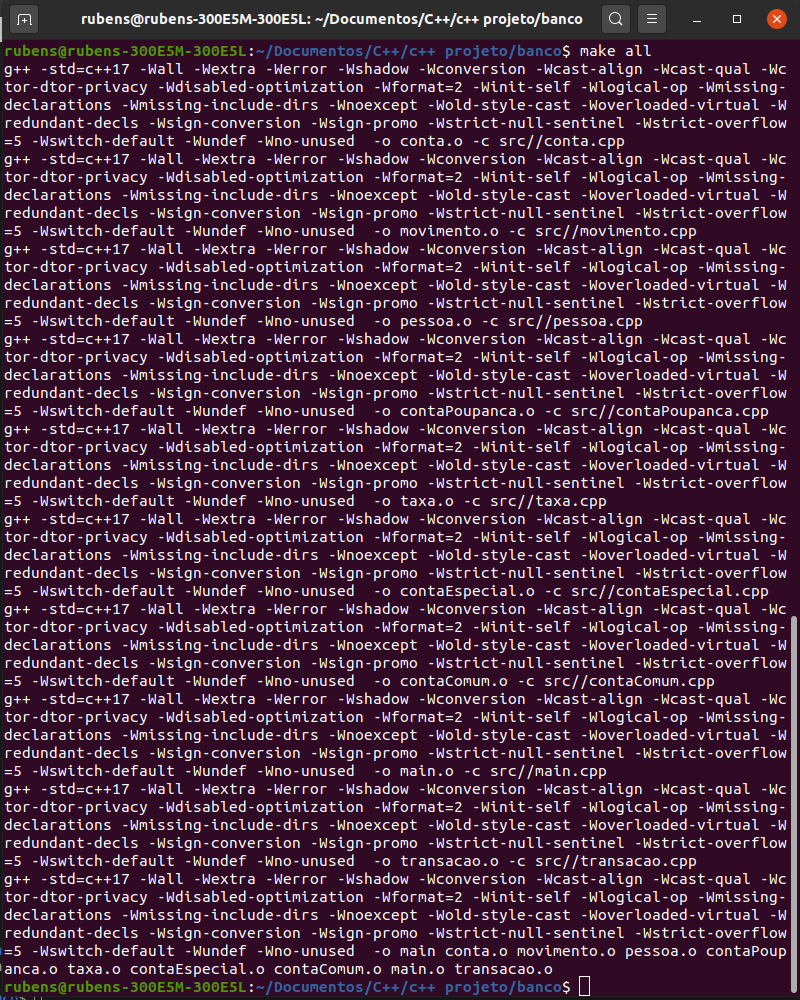
\includegraphics[width=8cm]{../img/compilando.png}
        \caption{Flags}
        \label{fig_Flags}
    \end{figure}

    Rodando o arquivo executável com o Valgrind

    \begin{figure}[htbp]
        \centering
        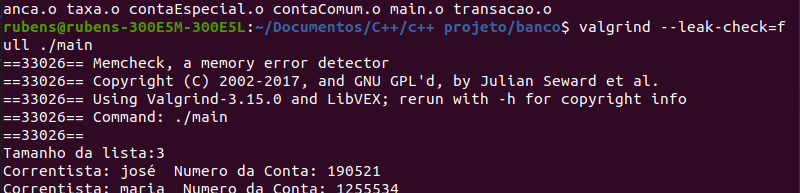
\includegraphics[width=8.8cm]{../img/valgrind1.png}
        \caption{Executando com o valgrind}
        \label{fig_valgrind1}
    \end{figure}

    \begin{figure}[htbp]
        \centering
        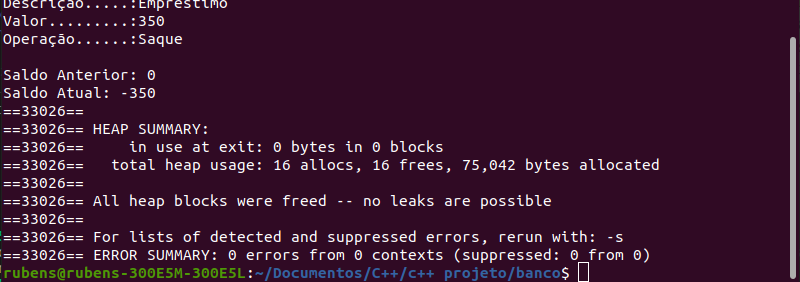
\includegraphics[width=8.8cm]{../img/valgrind2.png}
        \caption{Resultado da Analise}
        \label{fig_valgrind2}
    \end{figure}



\section{Conclusão}


O programa desenvolvido mostrou que atende todos os requisitos propostos, além de apresentar boa performace e atendendo às boas práticas de programação. Referente aos conceitos ensinados durante o semestre, o projeto foi essencial para o entendimento dos mesmos. 


\section{Referências}
[1] - Documentação Oficial C++ \url{http://www.cplusplus.com/}


[2] - Documentação Microsoft da linguagem C++ \url{https://docs.microsoft.com/pt-br/cpp/?view=msvc-160}


[3] - Wikilivros - \url{https://pt.wikibooks.org/wiki/Programar_em_C%2B%2B}

\end{document}